\documentclass[conference]{IEEEtran}

\usepackage[utf8]{inputenc}
\usepackage[T1]{fontenc}
\usepackage{lmodern}
\usepackage[spanish]{babel}
\usepackage{graphicx}
\usepackage{amsmath}
\usepackage{amssymb}
\usepackage{cite}
\usepackage{hyperref}
\usepackage{booktabs}

% Directorio de figuras: apunta a la carpeta figures/ local
% Para usar figuras de un experimento específico, copia o enlaza los PDFs aquí
\graphicspath{{figures/}}

% ---------------------------------------------------------------
\begin{document}

\title{Control de Formación de Robots Móviles Mediante Consenso}

\author{
  \IEEEauthorblockN{Leonardo Cárdenas}
  \IEEEauthorblockA{
    Departamento de Ingeniería\\
    Institución\\
    Ciudad, País\\
    correo@institucion.edu
  }
}

\maketitle

% ---------------------------------------------------------------
\begin{abstract}
En este trabajo se presenta un esquema de control de formación para múltiples robots móviles basado en algoritmos de consenso. Se estudian los casos de consenso con líder y consenso por promedio de errores, implementados sobre robots diferenciales en un entorno de simulación con Gazebo y ROS~2. Los resultados muestran convergencia de los seguidores a la trayectoria del líder bajo restricciones de velocidad impuestas mediante el algoritmo PVA.
\end{abstract}

\begin{IEEEkeywords}
control de formación, consenso, robots móviles, PVA, ROS~2
\end{IEEEkeywords}

% ---------------------------------------------------------------
\section{Introducción}

El control de formación de múltiples robots móviles ha atraído creciente interés debido a sus aplicaciones en vigilancia, exploración y transporte cooperativo~\cite{olfati2007consensus}. En este trabajo se adopta un enfoque basado en consenso distribuido, donde cada robot ajusta su velocidad en función de la información de sus vecinos dentro de un radio de percepción $R$.

% ---------------------------------------------------------------
\section{Planteamiento del Problema}

Considérese un grupo de $N$ robots móviles diferenciales cuya cinemática está dada por:
\begin{equation}
  \dot{x}_i = v_i \cos\theta_i, \quad
  \dot{y}_i = v_i \sin\theta_i, \quad
  \dot{\theta}_i = \omega_i,
  \label{eq:cinematica}
\end{equation}
donde $(x_i, y_i, \theta_i)$ es la posición y orientación del robot $i$, y $(v_i, \omega_i)$ son las velocidades de control.

% ---------------------------------------------------------------
\section{Algoritmo de Control}

\subsection{Consenso con Líder}

El robot líder sigue una secuencia de waypoints. Los seguidores implementan una ley de consenso:
\begin{equation}
  u_i^{\text{ref}} = k_1 \sum_{j \in \mathcal{N}_i} (q_j - q_i) + k_2 (q_L - q_i),
  \label{eq:consenso_lider}
\end{equation}
donde $\mathcal{N}_i$ es el conjunto de vecinos del robot $i$, $q_L$ es el estado del líder, y $k_1, k_2 > 0$ son ganancias de control.

\subsection{Restricciones PVA}

La velocidad de referencia $u_i^{\text{ref}}$ se proyecta al conjunto admisible definido por restricciones lineales de la forma $Av + Bw \leq C$, obteniendo la velocidad óptima $u_i^*$ más cercana a la referencia.

% ---------------------------------------------------------------
\section{Resultados}

\subsection{Configuración de la Simulación}

Las simulaciones se realizaron en Gazebo con $N$ robots diferenciales. Los parámetros utilizados se resumen en la Tabla~\ref{tab:params}.

\begin{table}[h]
  \centering
  \caption{Parámetros de simulación}
  \label{tab:params}
  \begin{tabular}{lll}
    \toprule
    Parámetro & Símbolo & Valor \\
    \midrule
    Número de robots    & $N$     & -- \\
    Radio de percepción & $R$     & -- m \\
    Ganancia 1          & $k_1$   & -- \\
    Ganancia 2          & $k_2$   & -- \\
    Velocidad máx.      & $v_{\max}$ & -- m/s \\
    Velocidad ang. máx. & $\omega_{\max}$ & -- rad/s \\
    \bottomrule
  \end{tabular}
\end{table}

\subsection{Trayectorias}

La Fig.~\ref{fig:trayectoria} muestra las trayectorias de todos los robots durante el experimento.

\begin{figure}[h]
  \centering
  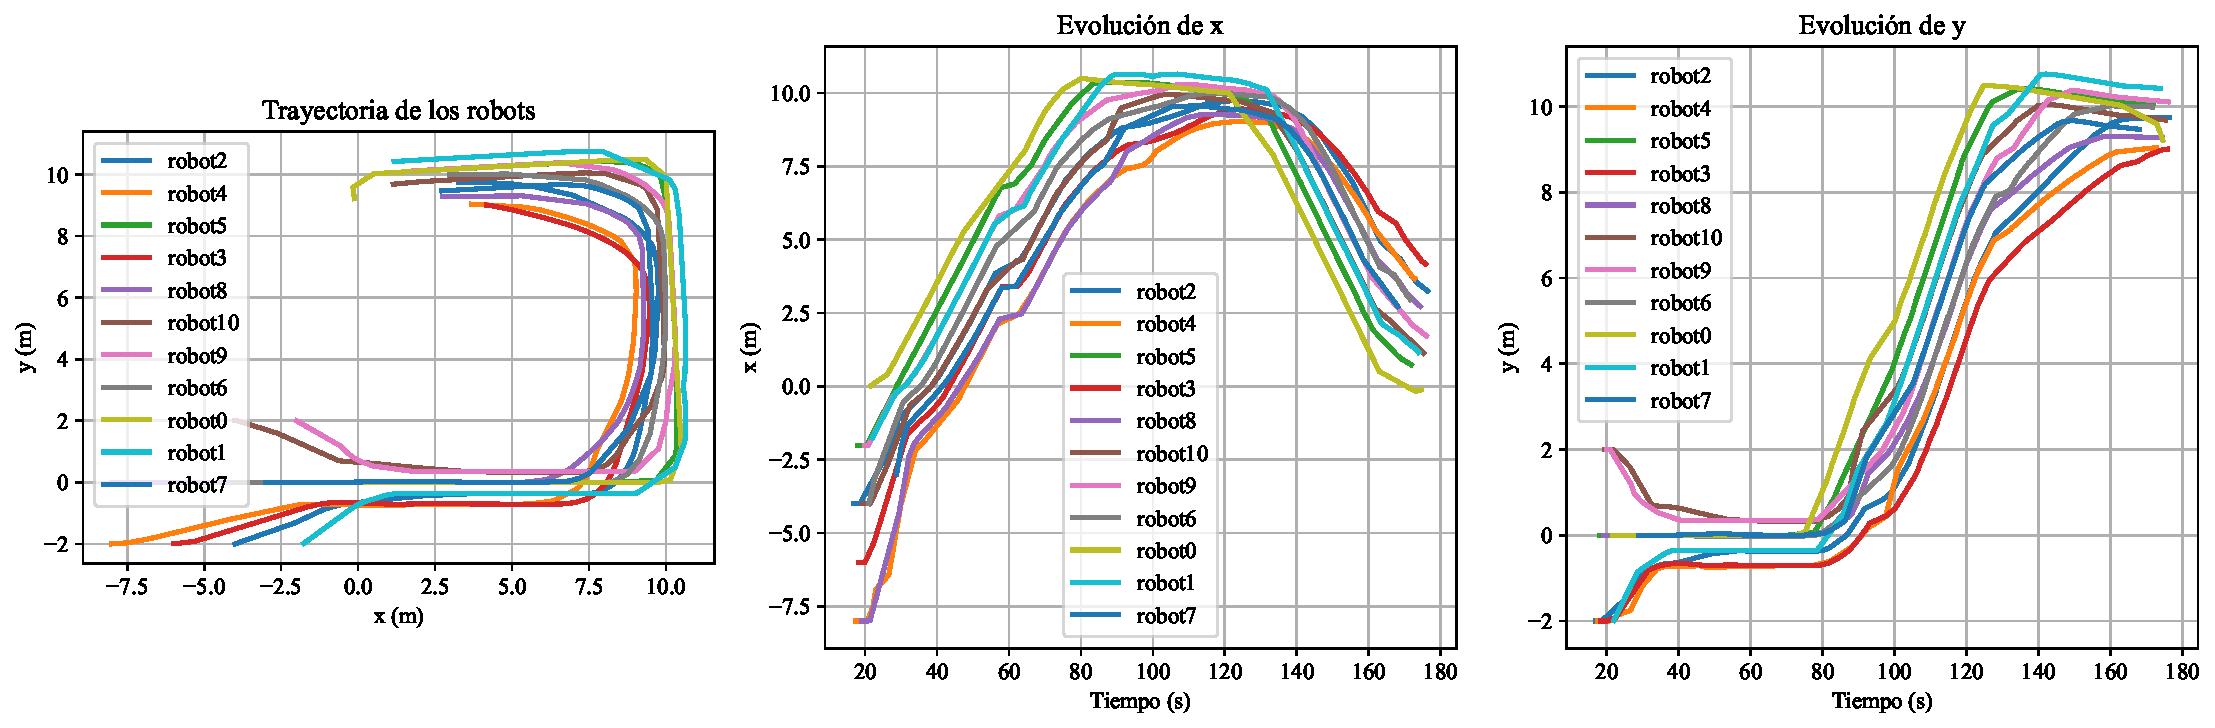
\includegraphics[width=\columnwidth]{resultados}
  \caption{Trayectorias, evolución de $x$ y evolución de $y$ de los robots.}
  \label{fig:trayectoria}
\end{figure}

% ---------------------------------------------------------------
\section{Conclusiones}

Se presentó un esquema de control de formación basado en consenso implementado en ROS~2. Los resultados de simulación demuestran que los robots seguidores convergen a la trayectoria del líder respetando las restricciones cinemáticas impuestas por el algoritmo PVA.

% ---------------------------------------------------------------
\bibliographystyle{IEEEtran}
\bibliography{references}

\end{document}